\documentclass[10pt]{article}
\usepackage[utf8]{inputenc}
\usepackage{amsmath}
\usepackage{amssymb}
\usepackage{graphicx}
\usepackage{hyperref}
\usepackage{menukeys}
\usepackage{nameref}
\title{openAPE}
\author{Stephan Unfried}
\date{\today} 
\begin{document}
\maketitle
\newpage
\tableofcontents
\newpage
\section{Introduction}
\section{project structure}
\subsection{Modules}
The project consists of tree parts, represented in tree maven modules. For details of the associations see figure \ref{fig:moduleuml}.
\begin{figure}[b]
\centering
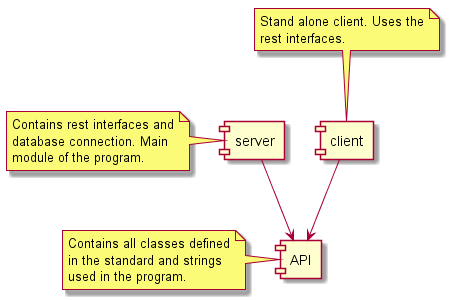
\includegraphics[width=0.8\textwidth]{uml/modulesuml.png}
\caption{module diagram.}
\label{fig:moduleuml}
\end{figure}
\subsection{API}
API contains classes and class structure used by the application server and clients who want to communicate with it. The classes contained in the API module represent the objects stored in the application. For clients it is important to uphold the class structure for the server to recognize those objects. For the structure of the module see figure \ref{fig:apiuml}.
\begin{figure}[b]
\centering
\makebox[\textwidth][c]{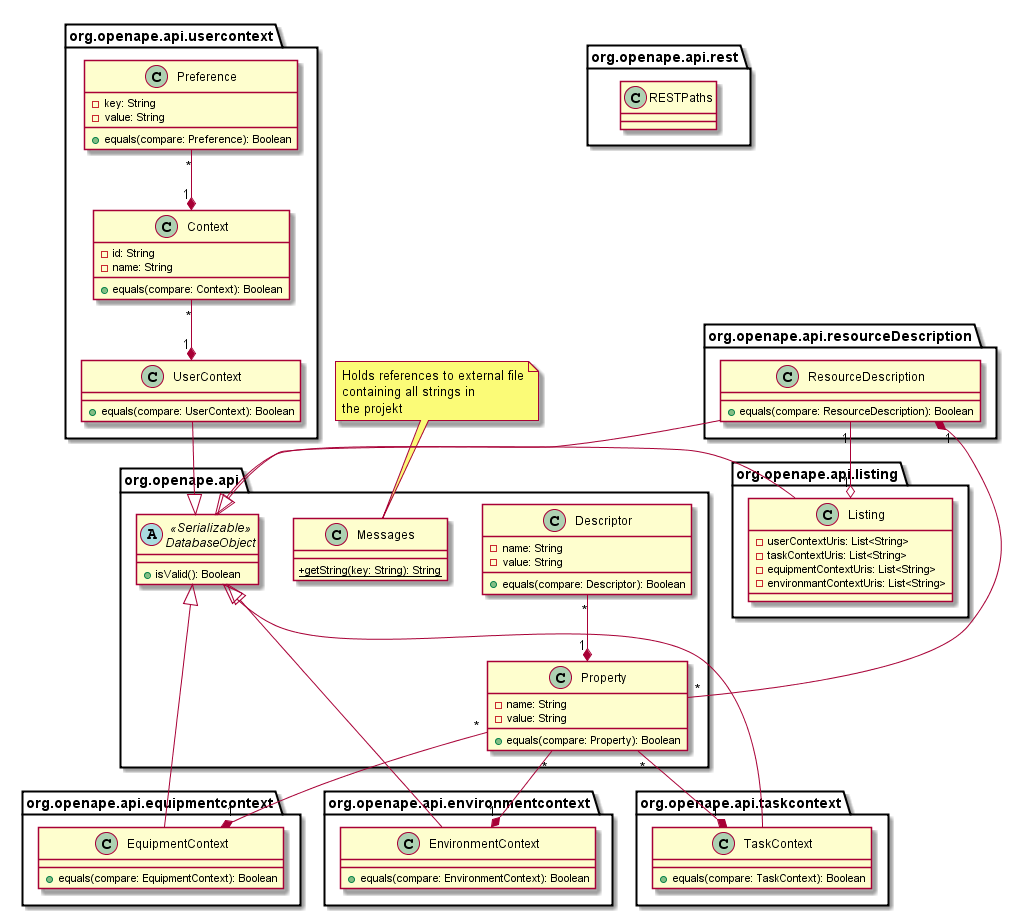
\includegraphics[width=1.4\textwidth]{uml/apiuml.png}}
\caption{API module structure diagram.}
\label{fig:apiuml}
\end{figure}
\subsection{Server}
The Server module is the main module of the application. It contains the web application used to up- and download contents. It provides an rest interface for access and uses a mongoDB and the file system to store data. The \emph{mongoDB} access can be configured in \directory{classes/config/mongo.properties}. For using the rest paths see the \emph{ISO-IEC\_CD\_24752-8} Standard. For the module structure see figure \ref{fig:serveruml}.
\begin{figure}[b]
\centering
\makebox[\textwidth][c]{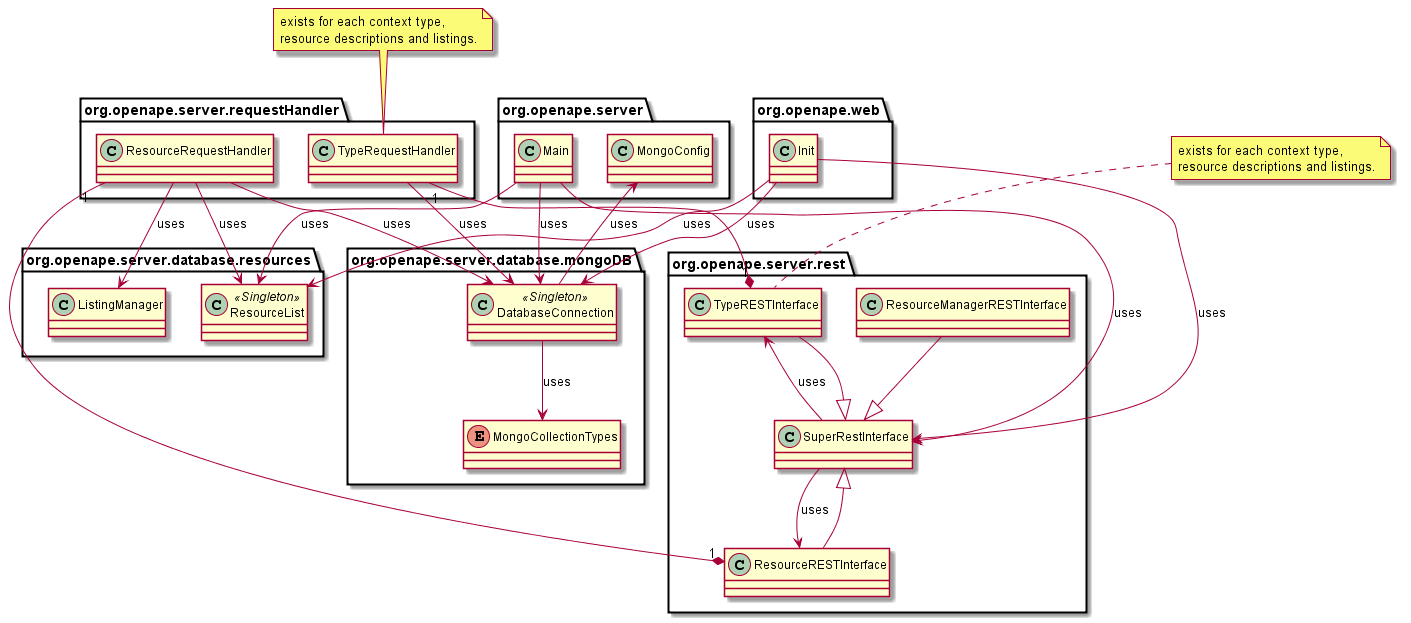
\includegraphics[width=1.5\textwidth]{uml/serveruml.png}}
\caption{Server module structure diagram.}
\label{fig:serveruml}
\end{figure}
\subsection{Client}
The Client is a sand alone module that uses the rest interface of the server to communicate with it. It can be replaced by any application capable of generating rest requests and processing the result.
\section{Get started with the project}
\subsection{remark} This section shows how to set up a development environment to work with the project. To see how to deploy the application for use please skip forward to section \nameref{sec:setupapp}.
\subsection{Github}
To use the repository used for this project you need a \emph{github} account and an application capable of running git commands.
\paragraph{Github account} To create an account visit the \href{https://github.com/}{github homepage}.
\paragraph{Github application} 
\section{Set up application}
\label{sec:setupapp}
\subsection{Set up MonoDB}
\subsection{Set up tomcat server}
\end{document}
